\documentclass[10pt,conference,compsocconf]{../IEEEtran}
\usepackage{xltxtra}
\usepackage{subfig}
\usepackage{booktabs}
\usepackage{flushend}
\usepackage[numbers,sort&compress]{natbib}
\setmainfont{Times New Roman}

\begin{document}

\title{idock 1.4: Further Improving Docking Speed over idock 1.0 and AutoDock Vina} % can use linebreaks \\ within to get better formatting as desired
\author
{
\IEEEauthorblockN
{
Hongjian Li, Kwong-Sak Leung and Man-Hon Wong
\IEEEauthorblockA
{
Department of Computer Science and Engineering, Chinese University of Hong Kong, Hong Kong, P.R. China\\
\{hjli, ksleung, mhwong\}@cse.cuhk.edu.hk
}
}
}
\maketitle

\begin{abstract}

In a previous study, we reported idock 1.0 for fast virtual screening and flexible ligand docking. In this study, we report idock 1.4, further improving the docking accuracy and docking speed. We carried out a comprehensive benchmark to better evaluate idock 1.4 and AutoDock Vina. Result showed that idock 1.4 outperformed AutoDock Vina by 10x in terms of docking speed. idock is free and open source, available at https://GitHub.com/HongjianLi/idock.

\end{abstract}

\section{Introduction}

As the X-ray crystallography technology evolves, more and more structures of biological macromolecules at atomic level have been revealed and deposited into the world's largest repository Protein Data Bank (PDB) \cite{539,537}. This rapid evolution catalyzes the development of various protein-ligand docking tools for structure-based drug discovery.

Protein-ligand docking is a method which predicts the preferred conformation of a small ligand when bound to a macro protein to form a stable complex. It also predicts the binding affinity in terms of free energy. The lower the free energy, the higher the binding affinity. Very often, the target protein is a viral enzyme of interest, and the small organic ligands that are predicted to inhibit the viral enzyme are what we want to discover. Structure-based virtual screening is simply a massive version of docking. It docks a database of drug-like ligands to a target, ranks them according to their predicted binding affinity, and shortlists the best ones for further investigation.

Among the many protein-ligand docking programs, AutoDock Vina \cite{595} (hereafter Vina for short) is a competitive one. It is free and open source. It runs faster than its predecessor AutoDock4 \cite{596} by an order of magnitude \cite{556}. First released in 2010, Vina has been cited by over 300 publications according to Google Scholar and adopted by quite many researchers \cite{609}, demonstrating its popularity.

\section{Motivation}

We developed idock 1.0, a multithreaded structure-based virtual screening tool for flexible ligand docking. It was capable of screening 1.3 drug-like ligands per CPU minute on average, making it a very competitive tool. Compared with Vina, idock 1.0 achieved a speedup of 3.3 in terms of CPU time and a speedup of 7.5 in terms of elapsed time on average. But even so, it still required about 10 hours on average to dock 10,928 drug-like ligands against a certain protein, not to mention massive docking of millions of ligands. Virtual screening remains a time-consuming practice. Faster algorithms and implementations are highly desired. We were motivated by the desire to provide built-in support for virtual screening and therefore developed idock. Moreover, we incorporated many implementation tricks to further speedup idock.

\section{Method}

The overall flowchart of idock.

Both idock and Vina share exactly the same scoring function, which is made up of a conformation-dependent part and a conformation-independent part. The conformation-dependent part is a weighted sum of five terms over all the pairs of atom $i$ and atom $j$ that can move relative to each other.

Both idock and Vina use Monte Carlo algorithm for global optimization and Broyden-Fletcher-Goldfarb-Shanno (BFGS) \cite{786} Quasi-Newton method for local optimization. A succession of steps consisting of a mutation and a BFGS local optimization are taken, with each step being accepted according to the Metropolis criterion.

idock automatically detects and deactivates inactive torsions, which are presented and activated in the input file in pdbqt format but have no impact on the overall scoring, such as \textemdash{OH} and \textemdash{NH$_2$}, because they only rotate the hydrogens.

idock invents its own thread pool in order to reuse threads and maintain a high CPU utilization throughout the entire screening procedure. The thread pool parallelizes the creation of grid maps and the execution of Monte Carlo tasks.

idock flattens Vina's tree-like recursive data structure of ligand into simple linear array structure to ensure a high data cache hit rate and easy coding.

idock accelerates the assignment of atom types by making use of residue information for receptor and branch information for ligand.

2-phase virtual screening

\section{Change Log}

Added program option config to allow users to specify a configuration file.
Added program option csv for dumping docking summary sorted in the ascending of predicted free energy.

intra-ligand free energy
Output predicted total free energy, predicted inter-ligand free energy and predicted intra-ligand free energy to docked PDBQT files. Output predicted free energy for each heavy atom to docked PDBQT files.

Added thread-safe progress bar
Added move constructors for several classes to boost performance.
Parallelized the precalculation of scoring function.
Automatic failover. Skipped already docked ligands.

12 docking examples
5 mainstream operating systems

Fixed a numerical bug when docking a ligand of only one single heavy atom.
Prevented dead loop by limiting the number of initial conformation trials.
Fixed a segmentation fault bug when the number of heavy atoms exceeds 100.

\section{Benchmarks and Results}

The experiments include 1) comparison of their redocking performance in terms of predicted conformations, and 2) comparison of their virtual screening performance in terms of execution time, memory usage, predicted free energy, and predicted conformations.

Vina x86 version 1.1.2 and idock x86\_64 version 1.4, the most recent versions of both programs at the moment these experiments were carried out, were used for experiments. Both programs were run on desktop computers with Intel Core i5-2400 CPU @ 3.10GHz and 4GB DDR3 RAM under Mac OS X 10.7.1 x86\_64.

\subsection{Benchmark of Conformation and Free Energy}

Two databases, PDBbind v2011 and CSAR NRC HiQ Set 24Sept2010

RMSD (Root Mean Square Deviation) values
Table \ref{tab:RMSD} shows the  between the crystal and docked conformations. 74\% RMSD values are below 2.0 \AA, a publicly accepted positive control for correct bound structure prediction.

\begin{table}
\centering
\begin{tabular*}
{\linewidth}
{@{\extracolsep{\fill}}ccccc}
\toprule
PDB ID & Protein & Ligand & Vina (\AA) & idock (\AA)\\
\midrule
2ZD1 & HIV RT & T27 & 0.465 & 0.555\\
1LI4 & SAHH   & NAD & 0.537 & 0.593\\
3IAR & ADA    & 3D1 & 0.605 & 0.569\\
3BGS & PNP    & DIH & 0.756 & 1.170\\
\bottomrule
\end{tabular*}
\caption{RMSDs between the crystal and docked conformations of T27, NAD, 3D1, and DIH predicted by Vina and idock.}
\label{tab:RMSD}
\end{table}

We picked several complexes and visualized their redocking results. Figure \ref{fig:Redocking} shows the four proteins in complex with their corresponding crystal and docked ligands. The ligands rendered in green are the crystal ones, the ligands rendered in red are the ones docked by Vina, and the ligands rendered in blue are the ones docked by idock.

\begin{figure}
\centering
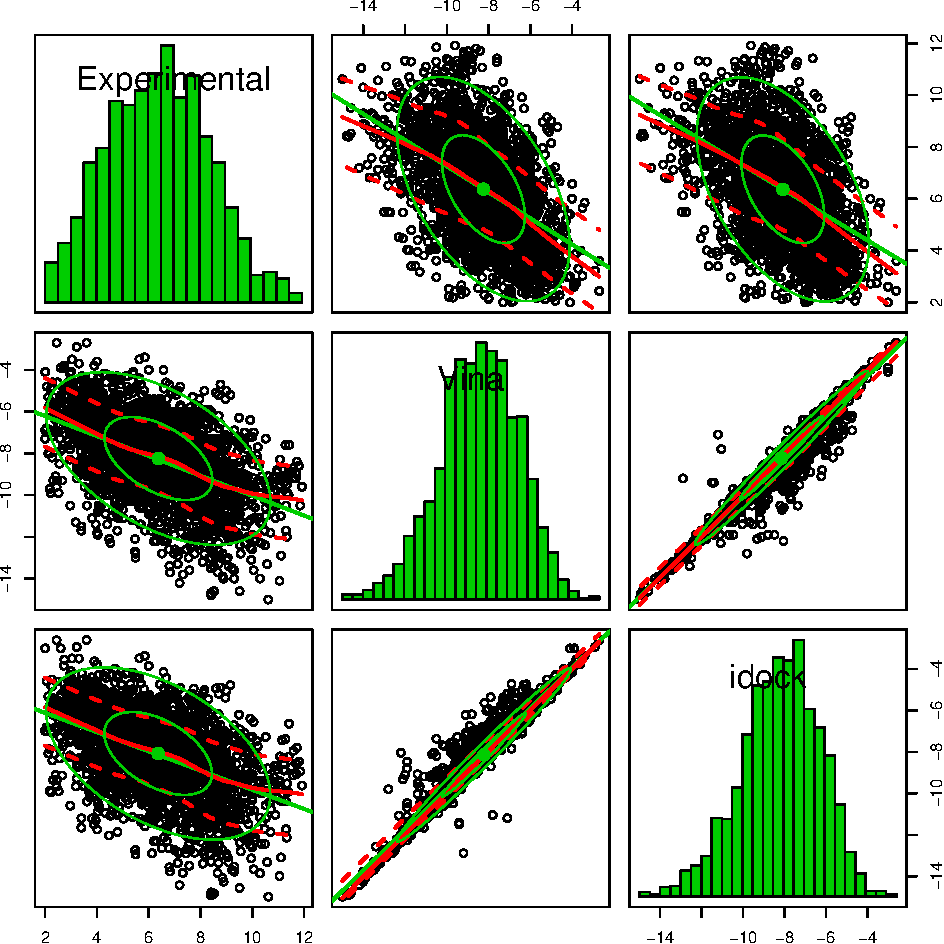
\includegraphics[width=\linewidth]{PDBbindFECorrelation.pdf}
\caption{Free energy correlation on PDBbind v2011.}
\label{PDBbindFECorrelation}
\end{figure}

\begin{figure}
\centering
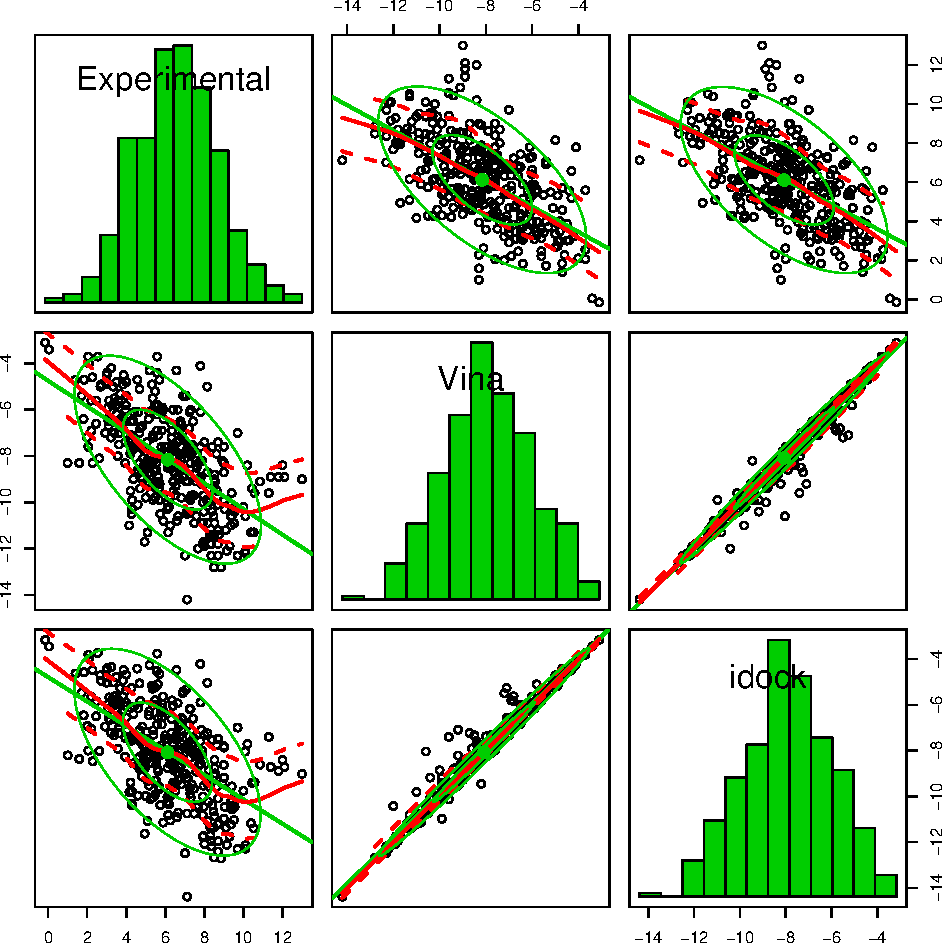
\includegraphics[width=\linewidth]{CSARFECorrelation.pdf}
\caption{Free energy correlation on CSAR NRC HiQ Set 24Sept2010.}
\label{PDBbindFECorrelation}
\end{figure}

\subsection{Benchmark of Virtual Screening Performance}

We collected 12 receptors from the PDB (Protein Data Bank) \cite{540,537}. They are 1HCL, 1J1B, 1LI4, 1V9U, 2IQH, 2XSK, 2ZD1, 2ZNL, 3BGS, 3H0W, 3IAR, and 3KFN.

1, 10, 100, 1000 ligands
[200, 300), [300, 400), [400, 500)
144 test cases in total.

ligands were collected from slice 16\_p0.0 of the clean drug like subset of the ZINC database \cite{532}.

\begin{figure*}
\centering
\subfloat
{
  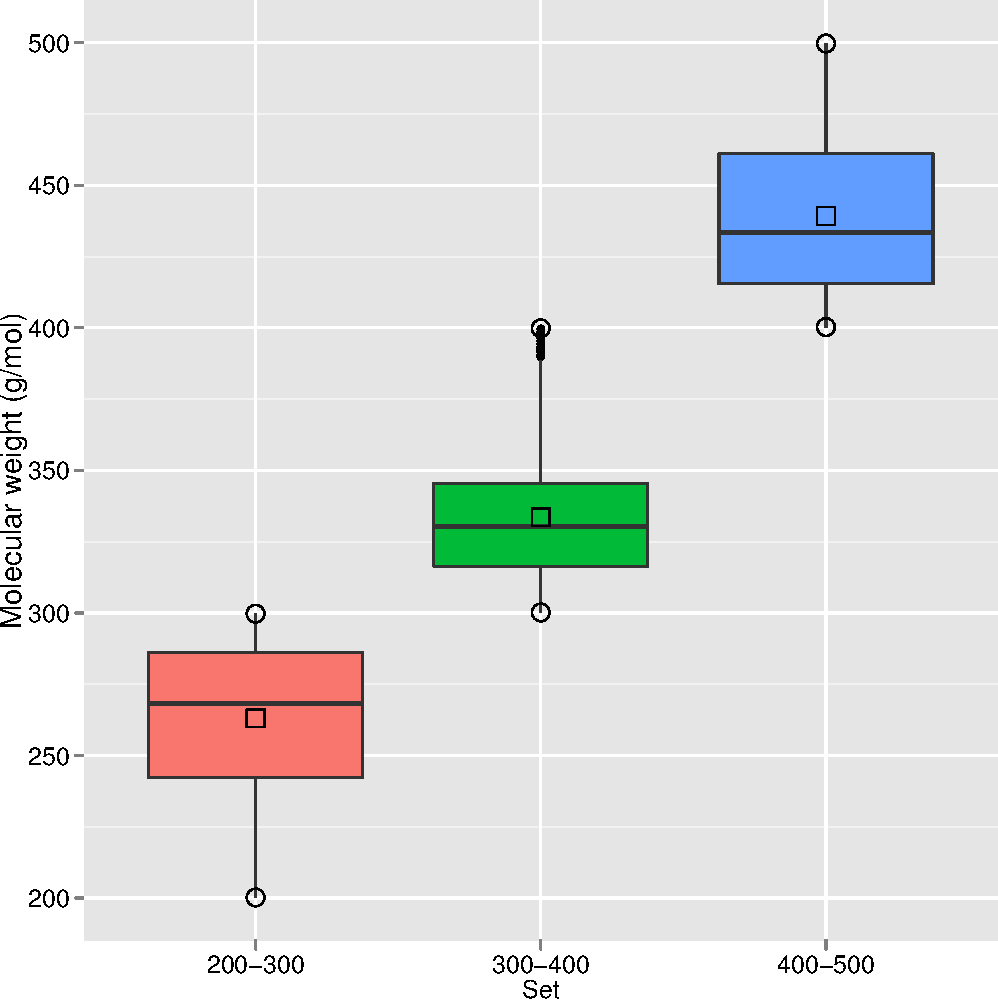
\includegraphics[width=0.485\linewidth]{MWT.pdf}
}
\subfloat
{
  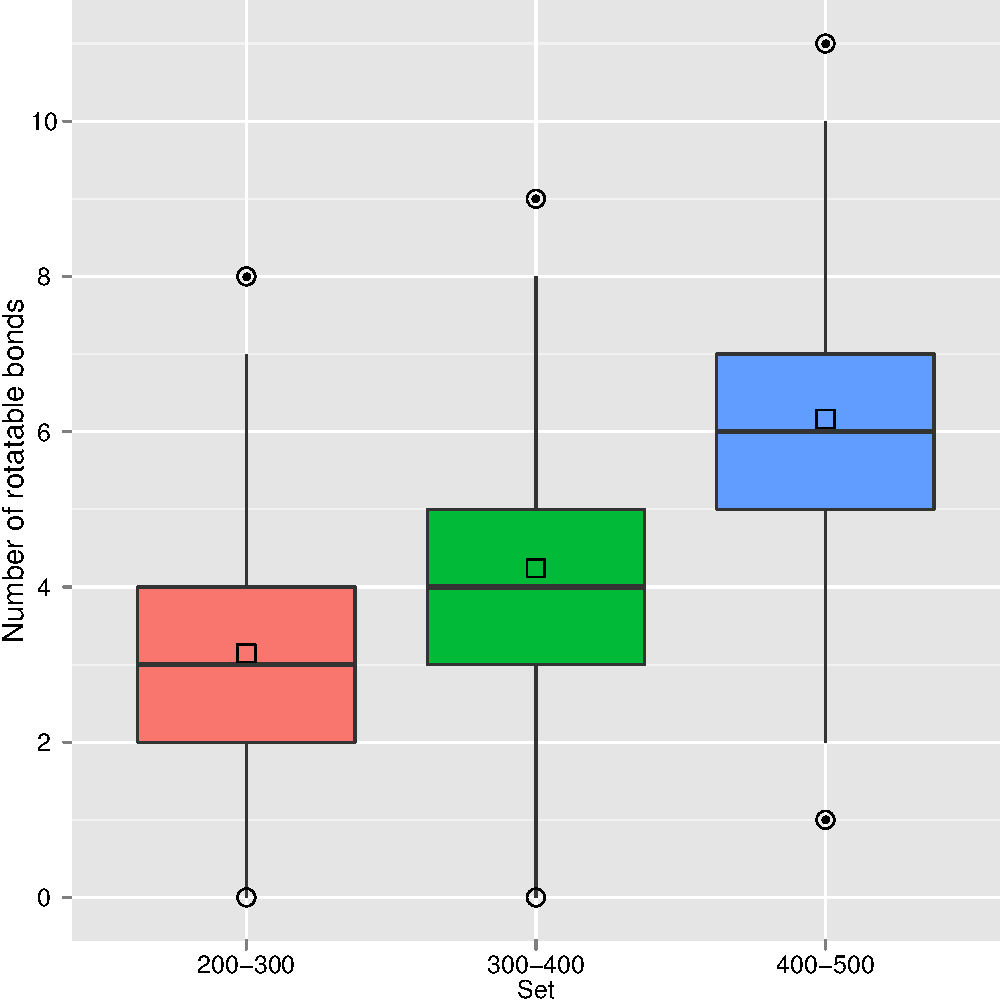
\includegraphics[width=0.485\linewidth]{NRB.pdf}
}
\caption{Boxplot of molecular weight and number of rotatable bonds of sets 200-300, 300-400, and 400-500.}
\label{MWT-NRB}
\end{figure*}

10,928 drug-like ligands were docked against the 12 proteins by Vina and idock. Since Vina can dock only one ligand in each run, a script containing 10,928 lines was generated and run instead, with each line being an execution of Vina to dock one individual ligand. Arguments to both programs were left as default. The GNU Time utility was used as profiler.

Table \ref{tab:ExecutionTimeAndMemoryUsage} compares the execution time and memory usage of both programs. Vina required 428 to 504 CPU hours for one protein case, while idock required merely 88 to 184 CPU hours, resulting in a speedup of 2.5 to 4.8 and a screening performance of 1.3 drug-like ligands per CPU minute on average. In terms of elapsed time, the speedup was increased to as high as 6.3 to 10.4 because idock better utilized the CPU cores thanks to its efficient thread pool. idock also better utilized available memory to build grid maps at a high resolution and retained them along the way. Even though idock consumed more memory than Vina, its maximum resident set size did not exceed 1.5 GB, hence idock can run be on mainstream desktop computers.

\begin{table}
\centering
\begin{tabular*}
{\linewidth}
{@{\extracolsep{\fill}}rrrrr}
\toprule
Program & CPU Hours & Elapsed & CPU Util. & Max Mem Usage\\
\midrule
\multicolumn{5}{l}{\textbf{HIV RT}}\\
Vina  & 464 & 69:15:13 &  670\% & 126 MB\\
idock & 162 & 10:57:46 & 1474\% & 856 MB\\
Ratio & 2.9 &      6.3 & 0.45   & 0.15\\
\noalign{\smallskip\smallskip}
\multicolumn{5}{l}{\textbf{SAHH}}\\
Vina  & 460 & 78:53:59 &  582\% &   150 MB\\
idock & 184 & 12:24:24 & 1484\% & 1,368 MB\\
Ratio & 2.5 &      6.4 &  0.39  & 0.11\\
\noalign{\smallskip\smallskip}
\multicolumn{5}{l}{\textbf{ADA}}\\
Vina  & 504 & 74:22:37 &  677\% & 114 MB\\
idock & 127 &  8:46:12 & 1452\% & 764 MB\\
Ratio & 4.0 &      8.5 &  0.47  & 0.15\\
\noalign{\smallskip\smallskip}
\multicolumn{5}{l}{\textbf{PNP}}\\
Vina  & 428 & 62:19:55 &  687\% & 116 MB\\
idock &  88 &  5:58:19 & 1479\% & 857 MB\\
Ratio & 4.8 &     10.4 &  0.46  & 0.13\\
\noalign{\smallskip\smallskip}
\multicolumn{5}{l}{\textbf{Average}}\\
Vina  & 464 & 71:12:56 &  654\% & 124 MB\\
idock & 140 &  9:31:40 & 1472\% & 961 MB\\
Ratio & 3.3 &      7.5 & 0.44   & 0.13\\
\bottomrule
\end{tabular*}
\caption{Execution time and memory usage of docking 10,928 drug-like ligands against HIV RT, SAHH, ADA, and PNP by Vina and idock. Maximum CPU utilization is 400\% due to Intel's Hyper-Threading technology.}
\label{tab:ExecutionTimeAndMemoryUsage}
\end{table}

Table \ref{tab:RMSEAndRMSD} summarizes the root mean square errors (RMSEs) of free energies and RMSDs of conformations predicted by both programs. The RMSEs of free energies predicted by both programs vary from 0.31 to 0.46 kcal/mol, apparently less than 2.85 kcal/mol, the standard error obtained by Vina, indicating both programs predicted very similar free energies. For 27\% to 40\% of all the 10,928 ligands, the RMSD of the conformations predicted by both programs is equal to or less than 1.0 \AA, and for 49\% to 61\%, the RMSD is equal to or less than 2.0 \AA, indicating both programs predicted similar conformations for around half of the cases.

\begin{table}
\centering
\begin{tabular*}
{\linewidth}
{@{\extracolsep{\fill}}cccc}
\toprule
Protein & RMSE (kcal/mol) & Avg RMSD (\AA) & RMSD $\leq$ 2.0 \AA\\
\midrule
HIV RT & 0.35 & 2.554 & 61\%\\
SAHH   & 0.46 & 4.190 & 49\%\\
ADA    & 0.33 & 2.620 & 59\%\\
PNP    & 0.31 & 2.966 & 53\%\\
\bottomrule
\end{tabular*}
\caption{RMSEs of free energies and RMSDs of conformations predicted by Vina and idock.}
\label{tab:RMSEAndRMSD}
\end{table}

\section{Discussion}

Vina supports flexible receptor docking by rotating flexible side-chains. However, we have not yet implemented flexible receptor docking into idock 1.4, so users who need this kind of docking should refer to Vina.

\section{Availability}

idock 1.4 is free and open source under Apache License 2.0 and available at https://github.com/HongjianLi/idock. Precompiled executables for 32-bit and 64-bit Linux, Windows, Mac OS X, FreeBSD and Solaris are provided. 12 docking examples and a doxygen file for generating API documentations are also provided.

\section{Future Directions}

We are developing istar, a SaaS (Software as a Service) platform for idock. The goal of istar is to automate virtual screening. Without tedious software installation, users, especially computational chemists, can submit jobs on the fly in either of three ways: 1) browsing our web site, 2) programming against our RESTful API, or 3) sending emails conforming to our specifications.

We will port idock to NVIDIA's GK104 GPU using CUDA and AMD's Tahiti GPU using OpenCL in order to harness their huge computational power and further speed up idock by at least an order of magnitude. We will also incorporate click chemistry into idock in order to computationally synthesize novel ligands.

\bibliographystyle{unsrtnat}
\bibliography{../refworks}

\end{document}
